\documentclass[11pt]{article}
\usepackage{fullpage}
\usepackage[margin=0.5in]{geometry}
\usepackage{amsmath,amssymb,amsfonts,graphicx,subfig,float,listings}
\renewcommand\vec[1]{\mathbf{#1}}
\usepackage{listings}
\usepackage[table]{xcolor}
\usepackage{framed,comment}
\newcommand\vx {\mathbf{x}}
\newcommand\vy {\mathbf{y}}
\newcommand\vb{\mathbf{b}}
\newcommand\vc{\mathbf{c}}
\newcommand\red[1]{\textcolor{red}{#1}}
\specialcomment{solution}{\bigskip\begin{leftbar}\par\noindent\textbf{Solution.} }{\end{leftbar} }
\excludecomment{solution}

\usepackage{color} %red, green, blue, yellow, cyan, magenta, black, white
\definecolor{mygreen}{RGB}{28,172,0} % color values Red, Green, Blue
\definecolor{mylilas}{RGB}{170,55,241}
\begin{document}

\lstset{language=Matlab,%
    %basicstyle=\color{red},
    breaklines=true,%
    morekeywords={matlab2tikz},
    keywordstyle=\color{blue},%
    morekeywords=[2]{1}, keywordstyle=[2]{\color{black}},
    identifierstyle=\color{black},%
    stringstyle=\color{mylilas},
    commentstyle=\color{mygreen},%
    showstringspaces=false,%without this there will be a symbol in the places where there is a space
    numbers=left,%
    numberstyle={\tiny \color{black}},% size of the numbers
    numbersep=9pt, % this defines how far the numbers are from the text
    emph=[1]{for,end,break},emphstyle=[1]\color{red}, %some words to emphasise
    %emph=[2]{word1,word2}, emphstyle=[2]{style},    
}

\begin{tabular}{l}
	\textbf{CSCI 5654-Fall16}: Assignment \# 4 \\
	\textbf{Your Name: Robert Werthman} \phantom{Supercalifragilisticexpialidocius Smith} \\
	\hline \\[10pt]
\end{tabular}

\noindent\textbf{P1.}
\bigskip

\noindent\textbf{(A)}
\\
Let $\max( 2 x_1 + 3 x_2 - 5 x_3,\ x_1,\ x_2,\ 2) \leq t$.  We can then form the following linear program:
\[\begin{array}{rllllll}
\min & t \\
\mathsf{s.t.} 
& +2x_1 & +3x_2 & -5x_3 & \leq t \\
& +2x_1 & -x_2 & +x_3 & \leq t \\
& x_1, & x_2 & & \leq t \\
\end{array}\]

\medskip 

\noindent\textbf{(B)}
\\
Let $t_1$, $t_2$, $t_3$, $t_4 \geq 0$. \\
Let $|x_1 + x_2| \leq t_1$, $| x_2 - x_3 | \leq t_2$, $| x_3 - x_1 | \leq t_3$, $| x_1 + x_2 + x_3 | \leq t_4$.\\
You now have the linear problem
\[\begin{array}{rllllll}
\min & +t_1 & +t_2 & +t_3 & +t_4 \\
\mathsf{s.t.} 
& +x_1 & +x_2 & & & \leq t_1 \\
& -x_1 & -x_2 & & & \leq t_1 \\
& & +x_2 & -x_3 & & \leq t_2 \\
& & -x_2 & +x_3 & & \leq t_2 \\
& -x_1 & & +x_3 & & \leq t_3 \\
& +x_1 & & -x_3 & & \leq t_3 \\
& +x_1 & +x_2 & +x_3 & & \leq t_3 \\
& -x_1 & -x_2 & -x_3 & & \leq t_3 \\
& t_1, & t_2 & t_3 & t_4 & \geq 0 \\
\end{array}\]

\medskip

\noindent\textbf{(C)}
\\
Let $\max( | x_1 | ,\ |x_2| ,\ |x_3|,\ |x_1+
  x_2 |) \leq t$. \\
You now have the linear problem
\[\begin{array}{rllllll}
\min & t \\
\mathsf{s.t.} 
& +x_1 & -x_2 & & \leq 5 \\
& & +x_2 & & \leq 3 \\
& +x_1 & & & \leq t \\
& -x_1 & & & \leq t \\
& & +x_2 & & \leq t \\
& & -x_2 & & \leq t \\
& & & +x_3 & \leq t \\
& & & -x_3 & \leq t \\
& +x_1 & +x_2 & & \leq t \\
& -x_1 & -x_2 & & \leq t \\
& t & & & \geq 0 \\
\end{array}\]


\bigskip
\newpage
\noindent\textbf{P2.}
\\
\lstinputlisting[basicstyle=\tiny]{p2.m}
\begin{center}
\begin{tabular}{|c|c|}
\hline
Coefficient & Value \\ \hline
$a_0$ & 8.704148513061227e-14 \\ \hline
$a_1$ & -3.375077994860476e-14 \\\hline
$a_2$ & -1.474376176702208e-13 \\\hline
$a_3$ & 2.131628207280301e-13 \\\hline
$a_4$ & -1.243449787580175e-13 \\\hline
$a_5$ & -1.056932319443149e-13 \\\hline
$a_6$ & 1.376676550535194e-13 \\\hline
$a_7$ & -3.979039320256561e-13 \\\hline
$a_8$ & 3.179678742526448e-13 \\\hline
$a_9$ & 6.430411758628907e-13 \\\hline
$a_{10}$ & 0.999999999999309 \\\hline
$b_0$ & 1.989519660128281e-13 \\\hline
$b_1$ & -2.060573933704291e-13 \\\hline
$b_2$ & 1.847411112976261e-13 \\\hline
$b_3$ & -8.526512829121202e-14 \\\hline
$b_4$ & -1.207922650792170e-13 \\\hline
$b_5$ & 7.815970093361102e-14 \\
\hline
\end{tabular}
\end{center}
\begin{figure}[H]
\centering
  \subfloat[Linear Regression Predictions]{
  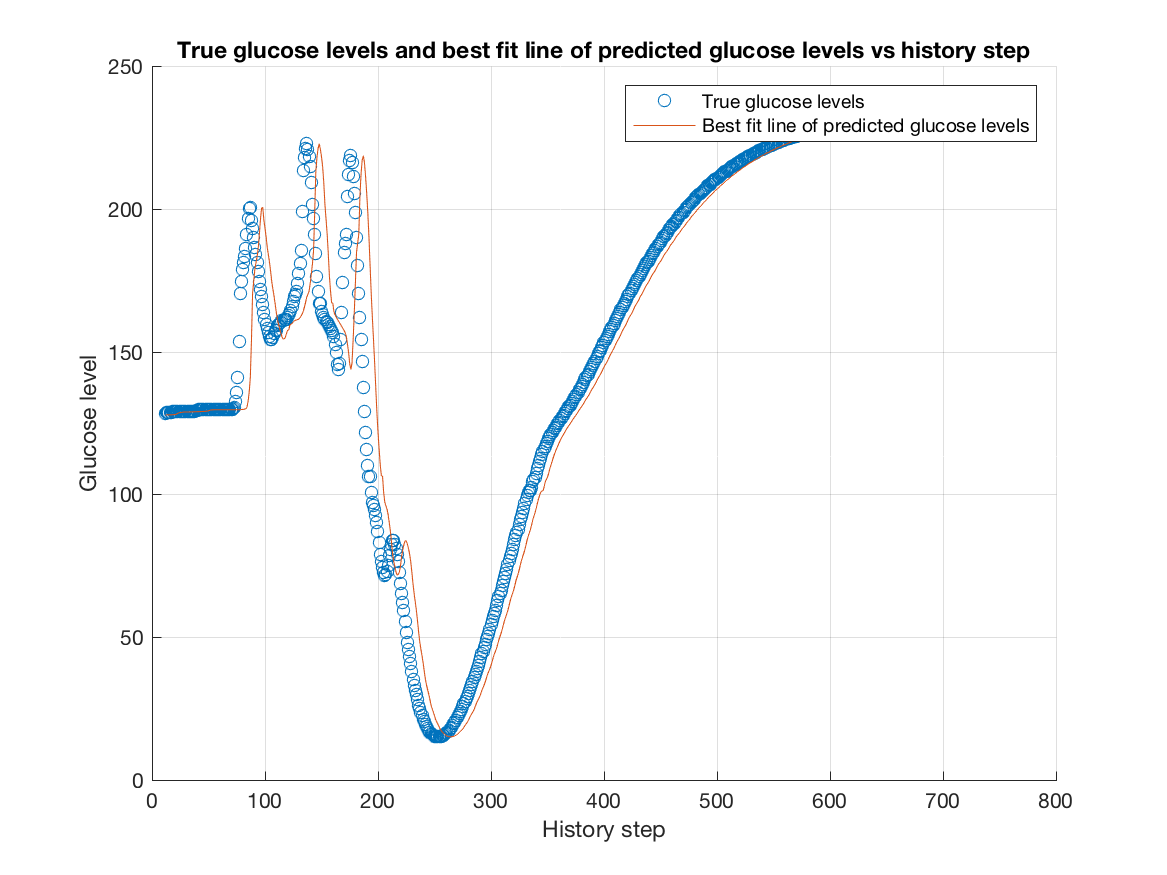
\includegraphics[scale=.6]{predictions.png}
  }
\end{figure}
\begin{figure}[H]
\centering
  \subfloat[Residuals]{
  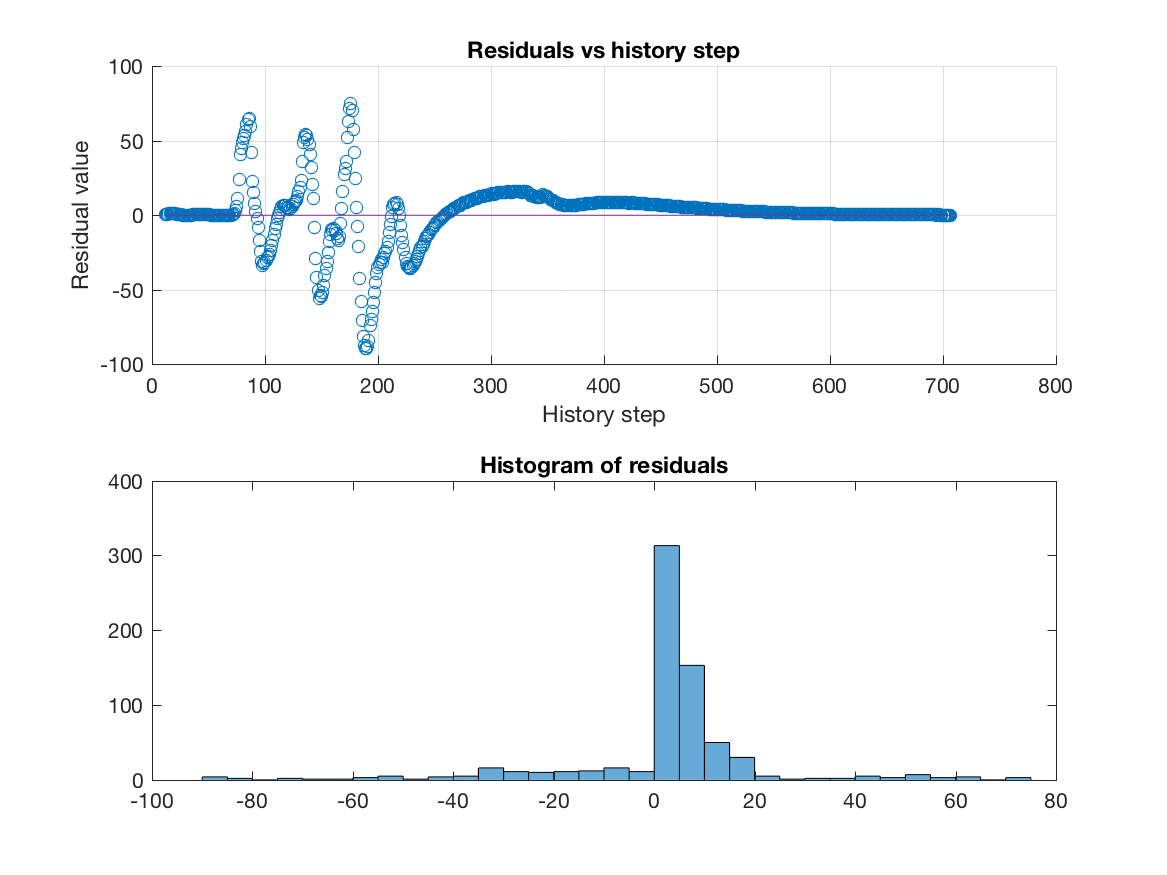
\includegraphics[scale=.5]{residuals.png}
  }
\end{figure}

\newpage

\noindent\textbf{P3.}\\

\noindent\textbf{(A)}

\begin{enumerate}
\item $\{ x_1, x_2, x_3, w_1, w_2, w_3 \}$.
  \[\begin{array}{r|ccccccccccccc}
  x_1 & +2 &  -x_4 & +x_5 & -x_6 & & & +w_{6}\\
  x_2 & -8 &  & +2x_5 & +x_6 & +w_{4} & +w_{5} & +w_{6} \\
  x_3 & +4 &  +x_4 & -2x_5 & & & -w_5 & -w_6 \\
  w_1 & -7 &  +x_4 & +x_5 & +3x_6 & +w_4 & +w_5 & & \\
  w_2 & -3 &  +2x_4 & & +x_6 & & & -w_6 \\
  w_3 & 2 &  +x_4 & -2x_5 & +x_6 & & -w_5 & -w_6 \\ 
  \hline
  \zeta & 16 & & -6x_5 & & -3w_4 & -2w_5 & -5w_6 \\
  \end{array}\]
\item $\{ x_1, x_2, x_5, w_3, w_5, w_6 \}$.
  \[\begin{array}{r|ccccccccccccc}
  x_1 & -1 & -x_3 & +x_4 & +2x_6 & -w_1 & & +w_4 \\ 
  x_2 & -4 & -x_3 & +x_4 & +x_6 & & & +w_4 \\
  x_5 & 0 & -x_3 & & +2x_6 & -w_1 & +w_2 & +w_4 \\
  w_3 & -2 & +x_3 & & +x_6 & & & & \\
  w_5 & 7 & +x_3 & -x_4 & -5x_6 & +2w_1 & -w_2 & -2w_4 \\
  w_6 & -3 & & 2x_4 & +x_6 & & -w_2 & & \\
  \hline
  \zeta & 14 & +4x_3 & -6x_4 & -6x_6 & +2w_1 & & -5w_4 \\
  \end{array}\]
\item $\{x_1, x_2, x_6, w_{4}, w_5, w_6 \}$.
  \[\begin{array}{r|ccccccccccccc}
  x_1 & -1 & & +x_4 & +x_5 & & -w_2 & & \\
  x_2 & -6 & +x_3 & +x_4 & +x_5 & +w_1 & -w_2 & -w_3 \\
  x_6 & 2 & -x_3 & & & & & +w_3 \\
  w_4 & -4 & +3x_3 & & +x_5 & +w_1 & -w_2 & -2w_3 \\
  w_5 & 5 & & -x_4 & -2x_5 & & +w_2 & -w_3 \\
  w_6 & -1 & -x_3 & +2x_4 & & & -w_2 & +w_3 \\
  \hline
  \zeta & 22 & -5x_3 & -6x_4 & -5x_5 & -3w_1 & +5w_2 & +4w_3 \\
  \end{array}\]
\end{enumerate}


\noindent\textbf{(B)} Perform one step of the revised simplex method for the dictionary with the basis:
\[ \{x_3, x_4, x_5, w_1, w_2, w_6 \} \]

\begin{enumerate}
\item Compute the constant column and objective rows of this dictionary.
  \[\begin{array}{r|ccccccccccccc}
  x_3 & 2 & & & -x_6 & +w_3 & & & \\
  x_4 & 6 & & +x_2 & -2x_6 & +w_3 & -w_4 & \\
  x_5 & 4 & -x_1 & & & -w_3 & & -w_5 \\
  w_1 & 3 & -x_1 & +x_2 & +x_6 & & & \\
  w_2 & 9 & -2x_1 & +x_2 & -2x_6 & & -w_4 & -w_5 \\
  w_6 & 0 & +2x_1 & +x_2 & -x_6 & +2w_3 & -w_4 & +w_5 \\
  \hline
  \zeta & -8 & -2x_1 & -4x_2 & +4x_6 & -2w_3 & +w_4 & \\
  \end{array}\]
\item Choose the entering variable with the largest coefficient.\\
\\
$x_6$ will be the entering variable because it has the largest coefficient.
\item Set up the equations to construct the column for the entering
  variable.\\
  \\
  The equation for the entering variable column $a_i$ is $a_i = -B^{-1}Ne_i$.

\item Choose the leaving variable.\\
\\
The leaving variable with be $w_6$ because it constrains the entering variable the most.
\item Write down the basic variables in the next dictionary.\\
\\
The basic variables will be $x_3,x_4,x_5,w_1,w_2,x_6$.
\end{enumerate}

\noindent\textbf{(C)}
\\
\[\begin{array}{r|ccccccccccccc}
x_5 & 1 & +x_1 & & & -x_4 & +w_2 & \\
x_6 & 4 & & +x_2 & +x_3 & -x_4 & & -w_4 \\
w_1 & 7 & -x_1 & +2x_2 & +x_3 & -x_4 & & -w_4 \\
w_3 & 2 & & +x_2 & +2x_3 & -x_4 & & -w_4 \\
w_5 & 1 & -2x_1 & -x_2 & -2x_3 & +2x_4 & -w_2 & +w_4 \\
w_6 & 1 & & +x_2 & +x_3 & +x_4 & -w_2 & -w_4 \\
\hline
\zeta & 4 & -2x_1 & -2x_2 & & -2x_4 & & -w_4 \\
\end{array}\]
\bigskip

\noindent\textbf{(D)}
\\
\textbf{No solution.}
\bigskip

\noindent\textbf{(E)} 
\\
\textbf{No solution.}
\bigskip
\lstinputlisting[basicstyle=\tiny]{p3.m}








\end{document}
